\documentclass{article}
\usepackage[utf8]{inputenc}
\usepackage[fencedCode]{markdown} 
\usepackage{hyperref}
\usepackage{indentfirst}
\usepackage{changepage}
\usepackage{amsmath}
\usepackage{forest}

\hypersetup{
    colorlinks,
    citecolor=black,
    filecolor=black,
    linkcolor=blue,
    urlcolor=blue
}

\begin{document}
\vspace{2in}
\title{A Brief Guide to Astrobee's Flight Software:\\
        Version 0.3}
\author{Keenan Albee\footnote{PhD Candidate and NASA Space Technology Research Fellow, Massachusetts Institute of Technology}, Monica Ekal\footnote{PhD Candidate, Portugal Instituto Superior Técnico}}
\date{July 2020}
\maketitle
\vfill
\begin{center}
This manual can be cited as:\\
K. Albee and M. Ekal, “A Brief Guide to Astrobee’s Flight Software,” 2020.
\end{center}
\newpage
This is a collection of user instructions, data, and software interfaces intended for researchers interested in interacting with NASA's Astrobee Flight Software. The guide is a work in progress, and is mainly intended for those interested in motion planning, estimation, and control, i.e., Guidance, Navigation, and Control (GNC). The guide is inspired by the SPHERES Guest Scientist Program Guide, originally published in 2009 to document the SPHERES free-flyer experiment. Do not rely on this information entirely for testing on-orbit; the guide is intended as a reference to find information and get working experiments without drowning in reading source code. There are also numerous Astrobee papers written by NASA Ames folks, which are good (but sometimes out-of-date) references \cite{Park2017a} \cite{Smith2016} \cite{Watterson2016} \cite{Fluckiger} \cite{Coltin2016a} \cite{Kim2017} \cite{Bualat2015} \cite{Lee2018}.
\\
\\
\indent Thanks to Brian Coltin, In Won Park, Marina Moreira, the Astrobee Ops Team, and others at NASA Ames IRG for their help in answering many questions.
\newpage

\tableofcontents

\newpage

\section{Setup, Building, and Running Code} 

Astrobee's public-facing, external code is available \href{https://github.com/nasa/astrobee}{here}. There are some guides available in that repo that will help you with getting the simulationup and running---the instructions in INSTALL.md specifically will help you with this. These instructions will provide some general guidance, but try out INSTALL.md first.

\subsection{Setup}
First, you need somewhere to put your source code, build directory, and install directory. The recommenced structure is shown in Figure \ref{fig:my_label}, where the source code cloned from NASA's GitHub is in \texttt{freeflyer-shared}. Most directories mentioned in this guide are relative to \texttt{freeflyer-shared}. (You can name this directory anything you want, \texttt{freeflyer-shared} is just a convention.)

A script is available to install required debians (packages)---check INSTALL.md for exact instructions. As a non-NASA user some of these packages (related to use of the Ground Data System (GDS)) are unavailable---this is okay, but you will notice that some packages are not found when running the installation scripts. The build must then be configured; essentially, you must run the configuration script with your desired build and install directories. Note that these paths are relative to \texttt{freeflyer-shared}:
\begin{markdown}
~~~~
./scripts/configure.sh -l -F -D -p $INSTALL_PATH -b $BUILD_PATH
~~~~

e.g.,

~~~~
./scripts/configure.sh -l -F -D -p ../freeflyer-install/native
-b ../freeflyer-build/native
~~~~
\end{markdown}

The recommended \texttt{\$INSTALL\_PATH} is \texttt{../freeflyer-install/native}. The recommended \texttt{\$BUILD\_PATH} is \texttt{../freeflyer-build/native}. 

\begin{figure}[h!]
    \centering
    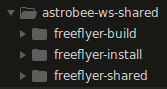
\includegraphics[height=80px]{img/folders.png}
    \caption{The recommended folder setup for Astrobee. This is slightly different from the normal catkin workspace structure you might be used to.}
    \label{fig:my_label}
\end{figure}

CMake has generated your makefile and other necessary bits in the build directory after running \texttt{configure.sh}.

\subsection{Building}

After setting up your directory structure and getting the source code, you can begin building (compiling and linking) your code. This process is a little different depending on whether you're working with the simulation or the actual robot (cross-compiling).

\subsubsection{For Simulation}
After setup, to incorporate new source code changes into the Astrobee build, run:
\begin{markdown}
~~~~
make -j2
~~~~
\end{markdown} 

\noindent{}in your build directory, \texttt{freeflyer-build/native/} for example.

What is the the build script doing? A few things---first, it checks to make sure a set of required libraries are installed. Some ROS messages are generated, media files are
loaded, and OGRE (a graphics engine used for some RViz visuals) is configured. Finally, C++ targets are built according to what is specified in the (long) Makefile in 
\texttt{freeflyer-build/native}. If you additionally want to install your targets, you can run:

\begin{markdown}
~~~~
make install -j2
~~~~
\end{markdown}

Build targets are placed in \texttt{freeflyer-install}, though this is not necessary for just working in simulation.

\subsubsection{For Hardware}

The cross-compile build to be uploaded to Astrobee hardware requires a bit of extra work in order to cross-compile ARM-compatible targets. Detailed instructions are in NASA\_INSTALL.md.

Directories for the chroot (mimicking the ARM file system) and toolchain (the actual tools used to cross-compile) must be specified. One option is to just put this working directory in the freeflyer workspace:

\begin{markdown}
~~~~
export ARMHF_CHROOT_DIR=$YOUR_CHOICE/arm_cross/rootfs
export ARMHF_TOOLCHAIN=$YOUR_CHOICE/arm_cross/toolchain/gcc
~~~~
\end{markdown}

NASA\_INSTALL.md details the further steps needed to do a cross-compile build for ARM. Those instructions are for NASA users only, however.

\subsection{Running}
The Astrobee ROS workspace environment must be overlaid for ROS to find it. This can be done by sourcing the workspace setup file:
\begin{markdown}
~~~~
source $BUILD_PATH/native/devel/setup.bash
~~~~
\end{markdown}

It is possible to interact from the command line using \texttt{rosrun} or \texttt{roslaunch} to start up sets of nodes. Astrobee uses ROS for most of its message-passing, so interacting like you normally would with a ROS environment is possible. It is also possible to launch a script that will run the desired ROS commands so that command line updates aren't required, or to write your own custom node the interacts with the desired topics. Again, Astrobee runs on ROS: the hard part is finding exact details on which nodes do what, and what their interfaces are.

One can also interact with Astrobee via NASA's ground data system (GDS) software. GDS is open-sourced, but its underlying DDS libraries are NASA-internal. GDS provides a GUI interface and convenient communications with Astrobee, and by default can support Guest Science interfacing with guest Android APKs or Java code.

\subsubsection{Sim Startup}

The sim.launch file located in the astrobee package is the starting point to run the simulation:

\begin{markdown}
~~~~
roslaunch astrobee sim.launch dds:=false robot:=sim_pub rviz:=true
~~~~
\end{markdown}

Default robot and dds arguments are required for non-NASA usage. Flags and more information can be found \href{https://github.com/nasa/astrobee/blob/master/simulation/sim_overview.md}{here}.

\subsubsection{Teleop}

A few mobility command-line commands can be issued using the Astrobee executive's teleop tool to directly control Astrobee. See the teleop tool documentation in \texttt{/management/executive/teleop\_tool.md}. These are convenience commands that sequence together other Astrobee tools to provide functionality for the user e.g., moving point to point by calling the planner and underlying control.

\subsubsection{Multiple Astrobees}

It is not immediately clear how to run multiple Astrobees at once. Would require namespacing nodes, cross-compilation must be separate for each robot if each is different.
TODO: document this process.

\section{Launch Sequence}

Astrobee is launched using a series of cascading launch files. The sequence of these launch files is given in Figure \ref{fig:launchfiles}. descriptions.launch creates the environment and corresponding frame transforms; spawn.launch starts artificial drivers and nodes running on the LLP and MLP; sim\_start.launch begins the Gazebo and RViz simulation environments. 

\begin{figure}[h!]
    \begin{adjustwidth}{-1in}{-1in}
    \centering
    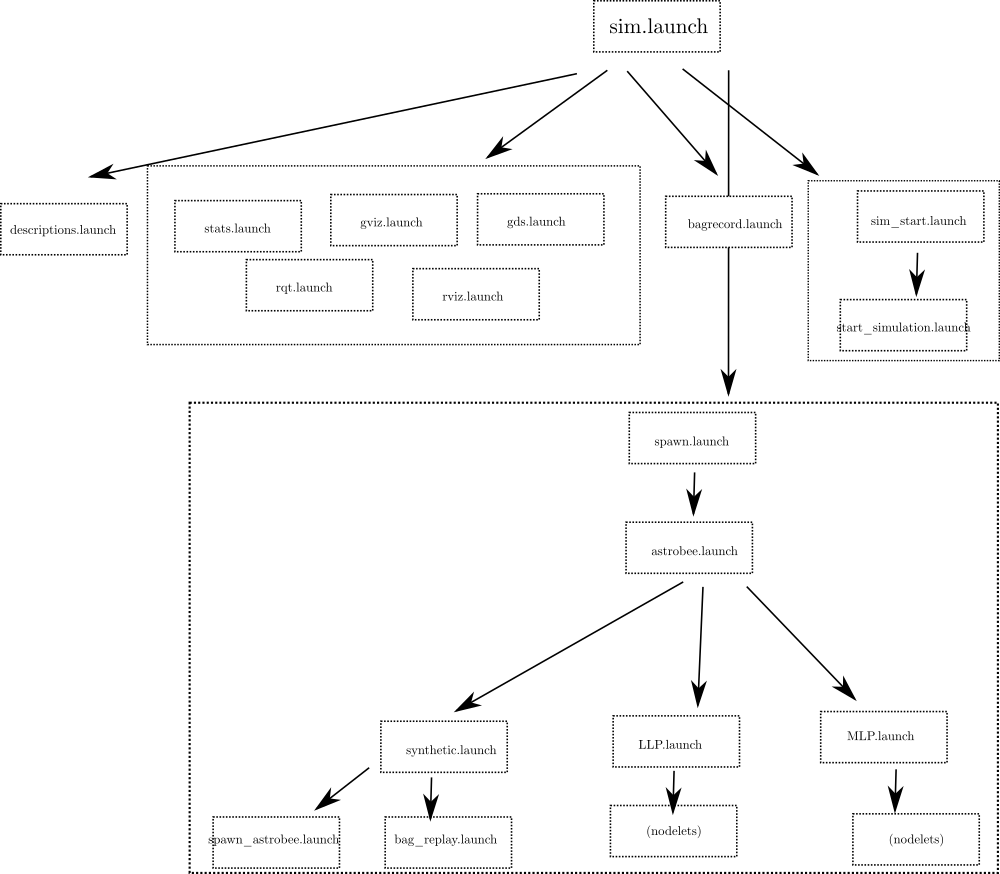
\includegraphics[width=1.4\textwidth]{img/astrobee2.png}
    \caption{The nominal Astrobee launch file sequence. The entrypoint to starting the simulation is sim.launch. A related launch file sequence is used to start up nodes on the actual hardware.}
    \label{fig:launchfiles}
    \end{adjustwidth}
\end{figure}

Consult individual launch files for more details. Most launch files are found in \texttt{astrobee/launch}, but some are also located in \texttt{simulation/launch}. Individual packages also usually have their own launch files. Note that Astrobee uses special nodelets instead of nodes, which are able to pass messages more efficiently. Documentation on nodelets can be found \href{http://wiki.ros.org/nodelet}{here}.

\section{Configuration}

A set of configuration files can be found in \texttt{astrobee/config}. These set many default robot parameters, some of which are reset via launch files. There is not very much documentation on these config files, but the inline coding is fairly self-explanatory. Some of the important physical characteristics are noted in this section. \texttt{astrobee/config/worlds} contains some particularly useful config information.

\subsection{Physical and Mass Properties}

In order to control the robot, it is necessary to know the system dynamics and parameters. Nominally, Astrobee obeys the rigid body dynamics of the Newton-Euler equations. Astrobee also has a small robotic arm, whose use results in free-flying dynamics. These dynamics are discussed in Chapter 3 of \cite{Albee2019}.

\subsubsection{Mass Properties}

Gazebo properties are set in their respective URDF files, specified in \\
\texttt{description/description/urdf}. The mass esimates are ``fairly accurate", the moment of inertia estimates are ``somewhat accurate". Values for ground air bearings are only ``somewhat accurate".
\\

The current mass estimate is $9.58\ $kg.
\\

The current inertia tensor estimate is
\begin{align*}
    I =  
    \begin{bmatrix}
              0.153 & 0 & 0\\
              0 & 0.143 & 0\\
              0 & 0 & 0.162
    \end{bmatrix}  \text{kg-m}^2\\
\end{align*}

\subsubsection{Position and Velocity Constraints}

Position constraints are not necessarily enforced by any default Astrobee planner. (planner\_qp, however, does obey the keep-in/keep-out zones, but not all of them.) These zones were originally specified in a json which is NASA-internal. \texttt{astrobee/resources/zones} has the latest ISS and granite table zones, written as serialized ROS messages. You will have to convert these back to message form to get the nominal position constraints.

By default, Astrobee uses a $0.1\ $m/s velocity constraint.

\subsubsection{Force and Torque Limits}

The quoted max thrusts per axis at various fan speeds are given in Table 1.

\begin{table}[h!]
\centering
\begin{tabular}{ |c|c|c|c| } 
    \hline
    Motor Speed (RPM)& x-axis (N)& y-axis (N)& z-axis (N) \\
    \hline
    2000 RPM & 0.452 & 0.216 & 0.257 \\
     \hline
    2500 RPM & 0.680 & 0.332 & 0.394 \\
     \hline
    2800 RPM & 0.849 & 0.406 & 0.486 \\
     \hline
\end{tabular}
     \label{table:speeds}
     \caption{The approximate thruster maximum forces per axis.}
\end{table}
     
TODO: thruster positions and limits per thruster and how to set this in sim. Mixing matrix. Astrobee diagram.
\\

Astrobee's thruster offset is about 0.1 m from the CoM, so the torque limit is very roughly about 1/10 of each of these values (each vent produces approximately half of the max force). These are only very rough guesses for the torque limits.

\subsection{Worlds}
By default Astrobee has two worlds, granite and ISS (International Space Station).
\begin{markdown}
**NOTE: If the simulation environment has been changed, the accelerometer bias must be reset. This can be done by running**

~~~~
rosrun executive teleop_tool -reset_bias
~~~~

**after starting the simulation.**
\end{markdown}


\subsubsection{Granite}
The granite table Ames uses is 2\ m x 2\ m. The coordinate system mimics that of the ISS, where z+ is toward GND, shown in Figure \ref{fig:sim_axes}.

\begin{figure}[h!]
    \centering
    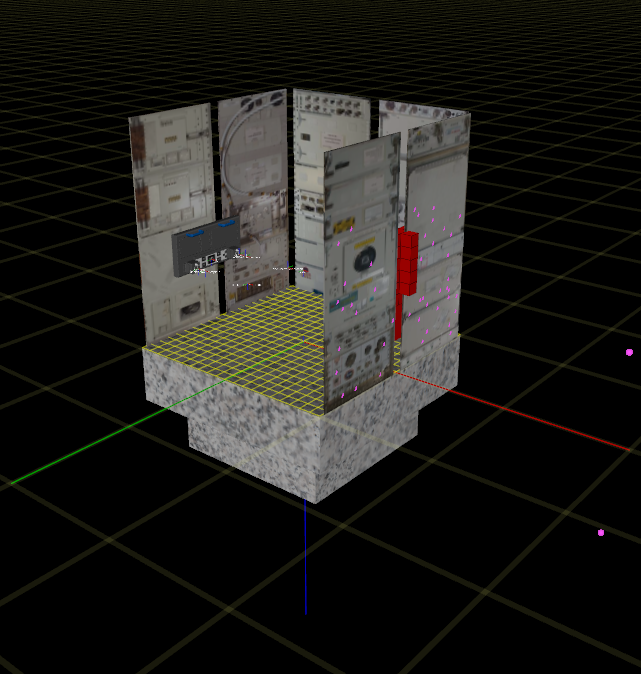
\includegraphics[width=0.8\textwidth]{img/sim_axes.png}
    \caption{The axis convention for simulation. RGB corresponds to XYZ.}
    \label{fig:sim_axes}
\end{figure}

\subsubsection{ISS}
The ISS world is a mockup of the US Segment of the International Space Station.

A good default location for the ISS world is:
\begin{markdown}
~~~~
roslaunch astrobee spawn.launch dds:=false
robot:=sim_pub pose:="11.25 -6.95 4.49 0 0 0 1" 
~~~~~
\end{markdown}

TODO: axis conventions, dimensions, imagery locations.


\section{Using Gazebo and the Sim}

Gazebo is the simulation backend (physics, visualization, etc.) used by the Astrobee simulator. It is tightly integrated with ROS and does not require any setup beyond setup steps followed in Section 1 and in INSTALL.md.

\subsection{Creating Objects}

The spawn\_astrobee node located in spawn\_astrobee.launch \\
(located in \texttt{/simulation/launch}) is used to bring Astrobee online in simulation, Figure \ref{fig:spawn}. Almost all information is specified via xacro files, which are kept in \texttt{description/description/urdf}. These xacros are converted to URDFs by a parameter command in astrobee.launch. The robot\_description parameter contains the output of this command and is passed to the spawn\_model script in \texttt{simulation/scripts/spawn\_model}. The launch sequence is summarized in Figure \ref{fig:spawn}. The model\_carriage* xacros are only used if specified by launch file input arguments. Documentation on URDF and Xacro files can be found \href{http://wiki.ros.org/urdf/XML}{here}.

\begin{figure}[h!]
    \begin{adjustwidth}{-0.5in}{-1in}
    \centering
    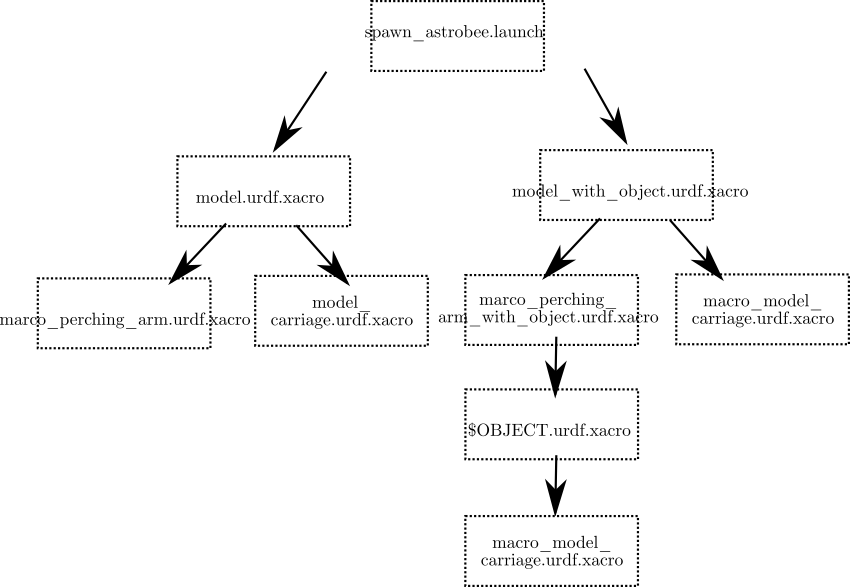
\includegraphics[width=1.3\textwidth]{img/astrobee4.png}
    \caption{The Astrobee object spawning sequence. This is used to create objects in the sim, and can be modified as desired.}
    \label{fig:spawn}
    \end{adjustwidth}
\end{figure}

\subsubsection{Attaching Rigid Objects}

Objects that are \textit{rigidly attached} to another model must have a URDF that is incorporated into the base. A sample launch sequence is available using sim\_info\_plan.launch. The object argument should be set to `empty', or the name of a desired URDF placed in \texttt{description/description/urdf}. Using model\_with\_object.urdf.xacro, this is accomplished through the perching arm, marco\_perching\_arm\_with\_object.urdf.xacro. Modifications to how the object is rigidly attached can be made in the `OBJECT' section at the bottom.

\subsubsection{Free-floating Objects}

Free-floating objects can be spawned using a custom xacro and do not require interfacing with model.urdf.xacro. Just ensure that the Gazebo spawn is called from the launch file sequence.

\subsubsection{Multiple Objects}

Multiple URDF files with the same link name are a problem. This can be fixed by creating an xacro macro that wraps the xacro file, allowing for different parents, etc. to be specified. This is currently used for model\_carriage.xacro, which must be used for both the supported object and Astrobee itself.

\subsubsection{Global Static Objects}

Ames uses a convention of ``global" transforms for objects that are static relative to the inertial ISS frame. Most of these objects are defined in \texttt{description/media/} and the ensuing subfolders. The actual transformations for these objects get set by the \texttt{framestore} node, which checks the config files (namely \texttt{iss.config} and \texttt{granite.config}) in order to set the necessary transformations relative to the ISS.

New global objects may be added to framestore for broadcasting, if desired.

\subsection{Visualization}

The Astrobee sim has RViz, SViz (Gazebo), GViz (GNC), and GDS visualizations. The RViz visualization is the most practically useful and is started up by visualizer.py. Each of these can be started using the launch file input arguments specified \href{https://github.com/nasa/astrobee/tree/master/simulation}{here}.
\\

\subsection{Multiple Astrobees}

Launching multiple Astrobees is possible using namespacing of topics. The Astrobee simulator can account for the following namespaces, currently: /, honey, bumble, and queen. '/' is the root namespace, and is the default for debugging.
\\\\
Many default Astrobee command-line tools accept the \texttt{-ns} argument, e.g.,\\
\begin{markdown}
`rosrun executive teleop -ns bumble -move -pos "4 0"`
\end{markdown}
\\\\
The spawn.launch launch file conjures up Astrobee in Gazebo and starts up namespaced nodelets. A namespaced Astrobee can be started using e.g.;\\
\begin{markdown}
`roslaunch astrobee spawn.launch ns:=honey pose:="2 0 4.8 0 0 0 1"`
\end{markdown}
\\\\
Additionally, spawn.launch namespacing options are available in the sim.launch file for calling up each platform, using args honey, bumble, and queen.

\subsubsection{Special Considerations}

By default, collisions between robots are \textit{not} considered!

\section{The Autonomy Pipeline}

The Astrobee GNC is divided into a few main packages: CTL (control), EKF (estimation), and FAM (force allocation module/mixer), along with packages for localization and planning. Locating the source files and identifying their inputs and outputs is key to making low-level modifications to Astrobee's autonomy software. By default, Astrobee launches a set of control and estimation nodelets (keywords: ctl, ekf, fam) on the LLP. (See LLP.launch.) Some higher-level nodes are launched on the MLP. (See MLP.launch.)

\subsection{Locations of Key Parts of the Autonomy Pipeline}
\begin{itemize}
 	\item High-Level Finite State Machine (FSM): \texttt{management/executive}
	\item Mobility FSM: \texttt{mobility/choreographer}
    \item Trajectory Planning: \texttt{mobility/planner\_*}
    \item Control: \texttt{gnc/ctl}
    \item Mixer: \texttt{gnc/fam}
    \item Estimation:  \texttt{gnc/ekf}
    \item Localization: \texttt{localization}
\end{itemize}

Most of the CTL, EKF, and FAM code was autocoded from a MATLAB Simulink model (and is therefore somewhat hard to read as source code). This Simulink model can be found in \texttt{gnc/matlab/astrobee\_control\_sim.slx}. Also note that most packages have individual READMEs with additional information.

\subsection{FSMs}

The executive and choreographer provide system-level and GNC-level management, respectively, often using their own FSMs to determine how to react. The exact logic behind decision-making is not covered here (it is extremely complex), but generally executive is useful from an autonomy perspective for getting external commands routed properly, and choreographer is useful for coordinating and monitoring interaction between GNC components (and interfacing with executive). Important information like inertial parameters and flight\_mode is also published by the choreographer.

\begin{figure}[h!]
	\centering
	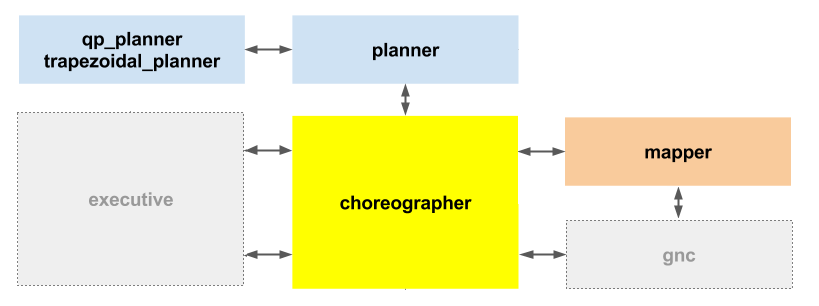
\includegraphics[width=1.0\textwidth]{img/mob_overview.png}
	\caption{A general overview of the interfacing between GNC components and the FSMs.}
\end{figure}

\subsection{Overriding the Planner}
\label{sec:plan}
Astrobee's default trajectory generators (planners) are natively coded in C++---there is no MATLAB autocoding. The goal of the planners is, given a goal state, to produce a set of dynamically-feasible trajectory setpoints. On top of that, the planners may optimize a cost function, or avoid obstacles. Only planner\_qp does either of these. The default planner, planner\_trapezoidal, creates straight-line trapezoidal velocity ramps and does simple obstacle checking---if an obstacle is in the way, it aborts. planner\_qp is a bit fancier, and produces minimum-jerk, smooth, obstacle-avoiding trajectories. There are two main ways to incorporate a new planner:

\noindent\textbf{Integrate into the Planner Framework - } This method requires the following:
\begin{itemize}
	\item Creating a new planner that inherits planner::PlannerImplementation (see planner\_trapezoidal\_nodelet.cc for an example)
	\item Filling in a minimal set of callbacks for a planner::PlannerImplementation
	\item Making sure planner.h is included, to register with the choreographer
\end{itemize}

A finite state machine running in the mobility subsystem (the choreographer) determines when and how planners are called, with configuration parameters also exposed via the rqt\_reconfigure ROS tool. Registration of a planner with the choreographer makes a planner accessible to the mob/motion action. mob/motion is \textit{the} interface for calling a planner. It is used by the teleop\_tool and by other internal commands involving motion requests.

\begin{markdown}
`/mob/motion` is aliased as `ACTION_MOBILITY_MOTION` in the codebase with action `ff_msgs::MotionAction`. This action is made available by the choreographer nodelet upon launch.
\end{markdown}

\begin{figure}[h!]
	\centering
	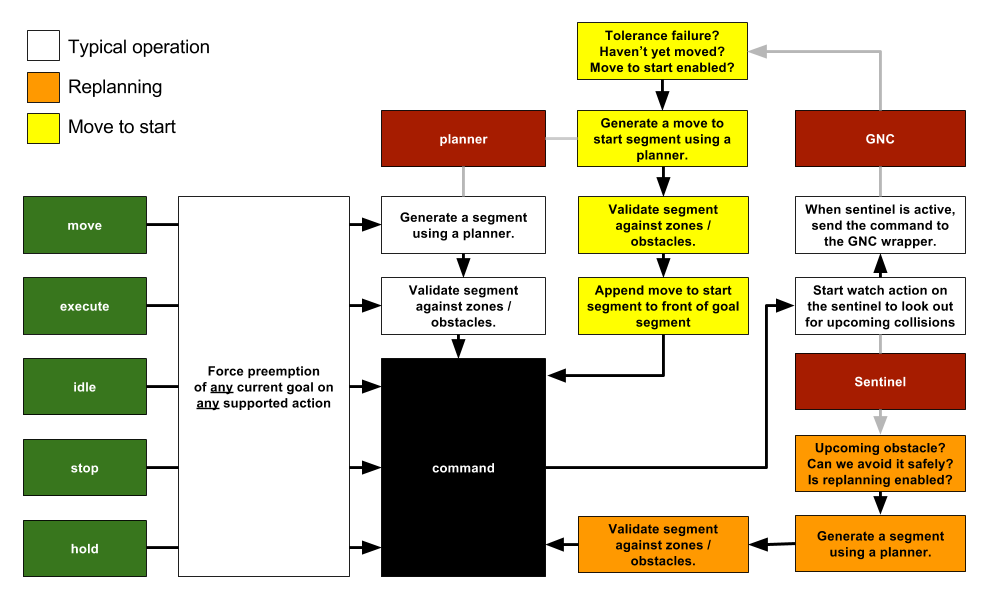
\includegraphics[width=1.0\textwidth]{img/choreographer.png}
	\caption{The default choreographer oversight of planning/control logic. MotionActions provide one of the 5 command types shown in green.}
\end{figure}

The flow of generating a trajectory and sending it out for control is:
\begin{itemize}
	\item teleop\_tool or executive calls choreographer.Plan() to initiate creating a trajectory (line 900 of choreographer\_nodelet.cc) via the MotionAction
	\item a request is sent to planner.SendGoal() (line 960 of choreographer\_nodelet.cc)
	\item the planner action server calls its GoalCallback() (line 252 of planner.h) and calls the PlanCallback() (line 267 of planner.h)
	\item the PlanCallback() routes the request to the trajectory generator defined by the planner implementation, and a plan\_result is set (e.g., line 85 of planner\_trapezoidal\_nodelet.cc)
	\item separately, a request for control is made in choreographer.Control() (line 1068 of choreographer\_nodelet.cc) which publishes a goal to the control client. This call is made by the FSM, but the exact mechanism for specifying the rate of reading the plan is not clear.
	\item ctl picks up the current action goal setpoint (line 343 of ctl.cc) and the segment is copied over to be processed.
	\item a wrapper around the autocoded GNC uses the setpoint and current state to compute the required forces and torques, and sends them to the FAM (line 438 of ctl.cc), see ctl.h for the wrapper class def. Note that Control() (line 400 of ctl.cc) actually sets the desired control state
\end{itemize}

\noindent\textbf{Bypass the Planner Framework - } It is also possible to bypass this framework entirely, if this acceptable for the Astrobee Ops team and your intended use. If you have your own trajectory generation scheme (in Astrobee parlance, a planner) you can avoid the FSM management of the choreographer by simply publishing your trajectory setpoints to the topic that the choreographer would have ultimately published to. 

The following publishers can be made with roscpp: one for base controller setpoints, and another for the arm controller. This will route trajectory setpoints directly to the controller monitoring TOPIC\_GNC\_CTL\_SETPOINT.
 
\begin{markdown}
~~~~
//  Publish setpoints to base controller
pub_ctl_ = nh->advertise<ff_msgs::ControlState>(
TOPIC_GNC_CTL_SETPOINT, 5, true);

//  Publish setpoints to arm
pub_arm_ = nh->advertise<sensor_msgs::JointState>(
TOPIC_BEHAVIORS_ARM_SETPOINT, 5, true);
~~~~

`/gnc/ctl/setpoint` is aliased as `TOPIC_GNC_CTL_SETPOINT` in the codebase with message `ff_msgs::ControlState`.
\end{markdown}

Anecdotally, sending commands too frequently can make ctl\_node zero out commanded force. There is also a position tolerance violation if tracking is particularly poor. Its value can be changed in the config files. This can lead to entering a different mode, `stopping' mode. Finally, you will need a way to run your setpoint publisher---in simulation, simply call via the command line; for ISS use, one possibility is creating a custom command sent from GDS.
\\

\subsection{Overriding the Controller (CTL)}

The ctl\_node handles determining force/torques to send to the force allocation module (FAM), given the state of the system and a desired nominal trajectory. Within the Simulink model, the closed loop control occurs at \texttt{astrobee/fsw\_lib/ctl\_controller/clc\_closed\_loop\_controller\_lib}.
The folllwing topics are used:

\subsubsection{Inputs}
\begin{markdown}
* `gnc/ekf`: State estimate from EKF.
* `gnc/ctl/control` Action. See the  [Control](@ref ff_msgs_Control) action specification for details.
\end{markdown}

\subsubsection{Outputs}
\begin{markdown}
* `gnc/ctl/command`: The force and torque commanded by control.
* `gnc/ctl/shaper`: The output from the GNC command shaper, which smooths the control.
* `gnc/ctl/traj`: The trajectory that the control subsystem is being commanded to follow.
* `gnc/ctl/segment`: The current segment the control subsystem is traversing.
* `gnc/ctl/progress`: The progress in executing the current segment.
\end{markdown}

\subsubsection{Overriding the Astrobee Controller Sequence}

If you don't care about integration with the Astrobee autonomy framework
framework (actions, state machines, etc) it's possible to publish directly to the controller or mixer (and arm, if desired) as seen in Section \ref{sec:plan}. The default controller can then be tweaked to use these setpoints as desired. However, the default controller is very opaque and challenging to interface with. More likely, it makes sense to take the setpoints, perform custom control, and write to the topic commanding the FAM.\\

\noindent\textbf{Overriding the Controller}
\\
\indent The following topics should be monitored:
\\
\begin{itemize}
	\item \texttt{TOPIC\_GNC\_CTL\_SETPOINT}, for setpoints to the base
	\item \texttt{TOPIC\_BEHAVIORS\_ARM\_SETPOINT}, for setpoints to the arm
\end{itemize}

\indent To send force and torque commands directly to FAM after the custom controller has calculated forces and torques, use:
\begin{markdown}
~~~~
//  Publish setpoints to fam
ctl_pub_ = nh->advertise<ff_msgs::FamCommand>(
TOPIC_GNC_CTL_COMMAND, 5);
~~~~
\end{markdown}

Take care to shut off the existing controller (node: ctl\_node), or to avoid writing to its input topic. \texttt{gnc/ctl/command} \textit{must} be updated at 62.5 Hz if overriding the stock controller, otherwise FAM will shut down the impeller system prematurely.


\subsection{Overriding the Mixer (FAM)}

It is also possible to override the mixer (FAM) by publishing directly to its write topics. If doing so, and you have already counted for shifted center of mass, you can disable the FAM's CoM shift adjustment by settting \texttt{/mob/inertia} 
to zero by modifying the Gazebo config file(s) in \texttt{astrobee/config/worlds}.

Note that the FAM Simulink can also be found at\\
\texttt{astrobee/fsw\_lib/ctl\_controller/clc\_closed\_loop\_controller\_lib}. Force and torque limits are also listed at \texttt{tun\_control\_linear\_force\_limit}, but must be verified.

\subsubsection{Inputs}
\begin{markdown}
* `gnc/ctl/command`: the control command which the FAM follows, containing force and torque. Force and torque are in the *body* frame. The mixer will account for an offset center of mass (CoM) by monitoring `mob/inertia` for the offset values.
\end{markdown}

\subsubsection{Outputs}
\begin{markdown}
* `hw/pmc/command`: The commands for the PMC to execute to obtain the desired force and torque.
\end{markdown}

\subsubsection{Notes on Overriding FAM}
\begin{markdown}
ctl.cc actually sets the force/torque values to take, `hw/pmc/command` gives the mixed version to hardware. The choreographer's flight\_mode message is used by FAM to determine PMC speed (see fam.cc). Actual actuation occurs in pmc\_actuator\_tool.cc. pmc\_actuator\_nodelet.cc is the real coordinator. Lots of complicated low-level commanding occurs there.

FAM defaults to a nominal fan setting in the following lines in fam.cc:

~~~~
// {
//   std::lock_guard<std::mutex> lock(mutex_speed_);
//   // Overwrite the speed command with the cached value, provided
//   // through the flight mode message offered by the choreographer
//   cmd->speed_gain_cmd = speed_;
// }
 ~~~~
 
You can set this nominal fan setting using flight\_mode, as follows:

~~~~
ros::Publisher pub_flight_mode_;
ff_msgs::FlightMode flight_mode_;
std::string flight_mode_name_ = "nominal";  // FlightMode to enter

ff_util::FlightUtil::GetFlightMode(flight_mode_, flight_mode_name_);
pub_flight_mode_ = nh->advertise<ff_msgs::FlightMode>(TOPIC_MOBILITY_FLIGHT_MODE, 1, true);
pub_flight_mode_.publish(flight_mode_);// Publish default flight mode
~~~~
\end{markdown}

\subsection{Overiding the Estimator (EKF)}

It is possible to run other estimators simultaneously (e.g. a parameter estimator using RLSE) or to replace the default estimator entirely. You can do what you wish with the results of additional computation.

\subsubsection{Inputs}
\begin{markdown}
* IMU Readings, `/hw/imu`: The IMU message. Must be received at a constant rate.
* Sparse Map Features, `/loc/ml/features` and `/loc/ml/registration`:
The features and registration pulses from the sparse map. The features include image coordinates and corresponding
3D feature positions from the map.
* AR Tag Features, `/loc/ar/features` and `/loc/ar/registration`: The same as the
sparse map features, but for AR tags. These are assumed to come from the dock camera.
* Optical Flow Features: `/loc/of/features` and `/loc/of/registration`: These
features are used for visual odometry. They are not associated with a 3D position, but are tracked over time
with a unique associated ID. Inside the EKF wrapper we keep track of these points over time and
send appropriate features to the EKF.
* Handrail Features: `/loc/handrail/features` and `/loc/handrail/registration`: The features for
localization with respect to the handrail. These are point features like with the sparse map features, but also
include a direction of the handrail axis and a boolean indicating whether the position along this axis has been observed.
\end{markdown}

\subsubsection{Outputs}
\begin{markdown}
* `/gnc/ekf`, the body state. See the EkfState message documentation for details.
* The body tf2 transform.
\end{markdown}

\subsubsection{Ground Truth}
Ground truth information is the ``true" physical state information about Astrobee. In simulation, this information is precisely known---in reality, it can only be estimated. Ground truth information can be found in:
\begin{markdown}
* Pose States, `/loc/truth/pose`, including position and attitude.
* Twist States, `/loc/truth/twist`, including velocity and angular velocity.
\end{markdown}
\subsubsection{Notes on Overriding EST}
The results of EST on actual hardware are likely worse, since feature points are generated for simulation purposes.

\section{The Arm}

Astrobee has a 2-joint perching arm which is controlled separately from the rigid body control. The arm's motion is treated as a ``behavior",
and is found in \texttt{behaviors/arm}. The documentation is fairly good, but essentially there are 3 layers of the arm software: firmware for the servos on a dedicated microcontroller; middleware to translate to/from serial commands and \texttt{sensor\_msgs::JointState} messages; and high-level action commands through the arm behavior using \texttt{ff\_msgs::ArmAction} messages. Figure \ref{fig:arm} explains this flow.
\\
\begin{figure}[h!]
    \centering
    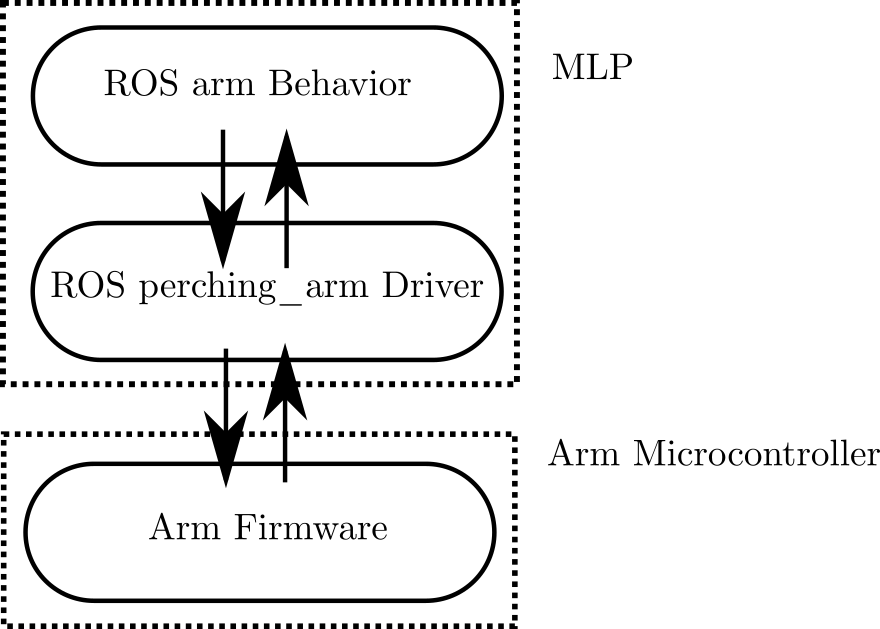
\includegraphics[width=0.8\textwidth]{img/arm_diag.png}
    \caption{The arm software flow.}
    \label{fig:arm}
\end{figure}
\\
\begin{markdown}
The possible actions are:

* ARM_STOP - Stop any action underway.
* ARM_DEPLOY - Deploy arm to pan = 0, tilt = 0.
* ARM_STOW - Stow arm back to its home position.
* ARM_PAN - Pan to a specific value in degrees.
* ARM_TILT - Tilt to a specific value in degrees.
* ARM_MOVE - Move to a specific pan and tilt value.
* GRIPPER_CALIBRATE - Instruct firmware to find gripper end-stops.
* GRIPPER_SET - Set the gripper to a percentage open.
* GRIPPER_OPEN - Open the gripper.
* GRIPPER_CLOSE - Close the gripper.

Note: Any payload must be started up via 

~~~~
eps_driver_tool -power -set on $PAYLOAD
~~~~

where `$PAYLOAD` is either `pay_ba` or `pay_ta`.
\end{markdown}

\subsection{Firmware}
\begin{markdown}
Located at `/submodules/avionics/src/tools/perching_arm`, this is NASA-only.
\end{markdown}

\subsection{Driver/Parser}
\begin{markdown}
Located at `/freeflyer/hardware/perching_arm`.

A command-line interface for serial commanding exists. Run 

~~~~
perching_arm_tester -o /dev/null
~~~~

to run the serial command-line interface.

* `m SERVO_NUM -DEG` moves SERVO_NUM to DEG degrees, [-90, 90]. Servo 0 starts at 90, Servo 1 starts at 0.
* `en g` enables the gripper
* `c 8 51 0` calibrates the gripper
* `c 8 52 0` opens the gripper
* `c 8 53 0` closes the gripper
\end{markdown}

\subsection{Command-Line Interface}
\begin{markdown}
There is a command line interface that can be used as follows:

~~~~
rosrun arm arm_tool -helpshort
~~~~

The arm's gripper must be calibrated before use. To calibrate the gripper, open it, close it and then set it to 50% open try the following sequence of commands:

    rosrun arm arm_tool -cal
    rosrun arm arm_tool -open
    rosrun arm arm_tool -close
    rosrun arm arm_tool -set 50
\end{markdown}


\subsection{Topics and Messages}

\begin{markdown}
At any point one can inspect the internal state of the arm behavior using the following command. The command will return a sequence of numbers, which represent a time ordered sequence of states. Please refer to ```ff_msgs::ArmState``` for a mapping from numbers to states.

~~~~
rostopic echo /beh/arm/state
~~~~

If you ever need to manually set the arm state to a specific value, you can call the ```set_state``` service with the new state as the single argument.

~~~~
rosservice call /beh/arm/set_state 1
~~~~
\end{markdown}

\section{Adding New Code}

This section includes general advice on pulling new code into the Astrobee build system and running it successfully in the simulation. (The process on hardware is similar, but has additional steps. Consult the Astrobee Operations Manual.)

\subsection{Adding a New Package}
\begin{markdown}
For non-NASA development, packages can be added in any directory in the `SOURCE_DIRECTORY`, e.g., `freeflyer-shared/develop`. New packages
can be added to the existing file structure of the sim, but the Makefile sequence must be modified to find them: use an `add_subdirectory` call.

You can make sure new packages get built by modifying the main `CMakeLists.txt`, located in `$SOURCE_DIRECTORY`:

Near the `if (USE_ROS)` conditional, add your desired subirectory, e.g. `add_subdirectory(develop)`

An additional `CMakeLists.txt` must be added in the newly created subdirectory. Using e.g. `gnc` as an example, format
an additional `CMakeLists.txt` in the newly added subdirectory. Place individual packages as `add_subdirectory($PACKAGE_NAME)` There are also many special CMake commands, include `INSTALL`, that will make sure your targets get put in the right place. This is usually not necessary for simulation, but consult the Astrobee Operations Manual for hardware testing.

Your new package name cannot compete with the name of an existing package! If this is the case, you must either replace the existing package's functionality
enitrely and turn off its compilation, or rename your package.
\end{markdown}

\subsection{Running a New Package}
\begin{markdown}
After a package gets compiled, its nodes and other targets are available for ROS use. It can be launched via `rosrun $PACKAGE $NODE_EXE_NAME`.
\end{markdown}

\subsection{Debugging}
\begin{markdown}
- `rqt_graph` is a handy ROS tool for showing node interactions.
- `rostopic echo` can show you what's being published on a certain topic.
- `rosnode $NODE info` can you show you what a node is interacting with.
- logging using `ROS_NODELET_DEBUG` statements is especially handy for viewing output. See the Section below on Nodelet Debugging and Logging.
\end{markdown}

\subsection{``Turning Off" a Node}
\begin{markdown}
You can effectively "turn off" a node by stopping its execution from the Astrobee launch file sequence. To do so,
trace the launch file calls from `astrobee/launch` (see Section 2) relevant to your current usage and remove your node from execution.

To stop compilation entirely, your node's package must be removed from the chain of `CMakeLists.txt`'s.

Alternately, you can just run `rosnode kill $NODE`.
\end{markdown}

\subsection{Killable Astrobee Nodes}
\begin{markdown}
A convenient way to start Astrobee and kill it without restarting the entire simulation is to set `default` to `False`
in `sim.launch`. Then, in a separate terminal, launch `spawn.launch`. Be sure to use the same arguments you would use for launching the sim, e.g:

`roslaunch astrobee spawn.launch dds:=false robot:=sim_pub`
\end{markdown}

\subsection{The Astrobee Build System}

\subsubsection{Comparison to catkin}

A typical catkin workspace will look like the following:

\begin{figure}[h!]
	\centering
	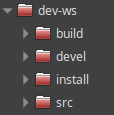
\includegraphics[]{img/typical-ws.png}
\end{figure}

Meanwhile, the Astrobee workspace looks like the following:

\begin{figure}[h!]
	\centering
	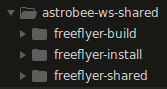
\includegraphics[]{img/folders.png}
\end{figure}
\vspace{1cm}

catkin is normally used to produce the ROS workspace, and then to manage CMake in compiling files from src in build, and moving the products to devel and install. Astrobee's build system will place the devel folder inside freeflyer-build, and a few custom CMake scripts exist for e.g., installation of launch files. The Astrobee build process, documented in Section 1, uses regular \texttt{make} called from the freeflyer-build folder. Rules defined in the top-level \texttt{CMakeLists.txt} in src make sure that some catkin-specific functions are fulfilled.


\subsubsection{CMake}
The /cmake folder has custom Cmake functions that are used in the top-level CMakeLists.txt and its sub-CMakeLists.txt's. The important ones to note are: \texttt{CreateLibrary}, \texttt{CreateMsgTargets}, and \texttt{InstallLaunchFiles}. These custom commands are listed below, to ensure that any code you write actually gets placed in the correct directories that ROS and Astrobee hardware will expect to see.

\subsubsection{ROS Messages}

The majority of Astrobee's message files are located in the ff\_msgs package, located at\\\\
\texttt{communications/ff\_msgs/msg/}\\

During build, these .msg files get ROS-ified and turned into usable headers for C++. Include these in your source files, e.g., \texttt{\#include <ff\_msgs/FamCommand.h>}. \\

Custom messages in a package can be installed using\\\\
\texttt{create\_msg\_targets()}

\subsubsection{Launch Files}

Custom launch files in a package can be installed using\\\\
\texttt{install\_launch\_files()}

\subsection{Nodelets}

Nodelets incur no copy-passing and can therefore be more efficient than nodes. Astrobee uses them. More information on nodelets can be found \href{http://wiki.ros.org/nodelet}{here}. Nodelets have a \textit{manager} which can handle multiple nodelets and takes care of the no-copy message passing between nodelets under that manager. You must roslaunch both a nodelet and its manager for your code to run. (One exception: it is possible to launch standalone nodelets, mainly for debugging)

\textbf{Integrating a Nodelet}
The following must be included and/or modified in your package:
\begin{itemize}
	\item nodelet\_plugins.xml : add and fill out basic information
	\item package.xml : add a nodelet dependency
	\item CMakeLists.txt : create a shared library
	\item src : extend the NodeHandle class and include required functions in your source code. For Astrobee, all nodelets extend from ff\_util::FreeFlyerNodelet.
	\item launchfile : your main launchfile (probably MLP.launch or LLP.launch) must call your nodelet and nodelet manager to start them. See MLP.launch for Astrobee-esque examples.
\end{itemize}

Here is an example of creating a shared library for your nodelet within \texttt{CMakeLists.txt}:
\begin{markdown}
	~~~~
	create_library(TARGET tumble_targ_ctl
	LIBS ${catkin_LIBRARIES} ${EIGEN_LIBRARIES} common ff_nodelet
	INC ${catkin_INCLUDE_DIRS} ${EIGEN3_INCLUDE_DIRS}
	DEPS ff_msgs ff_hw_msgs)
	~~~~
\end{markdown}

\textbf{Nodelet Debugging}
It is useful to run nodelets individually for debugging purposes. This can be done with a special launch file that launches the nodelet \textit{standalone}, without a nodelet manager, or with a nodelet manager just like in MLP.launch. You \textit{must} set your environment variables to be the same as those used in astrobee/sim.launch, since they will be used by FreeFlyerNodelet. Additionally, logging must be set appropriately as noted in the next section. For example,
\begin{markdown}
	<launch>
	<arg name="robot" default="$(optenv ASTROBEE_ROBOT sim)" />
	<arg name="world" default="$(optenv ASTROBEE_WORLD iss)" />
	
	<env name="ASTROBEE_ROBOT" value="$(arg robot)" />
	<env name="ASTROBEE_WORLD" value="$(arg world)" />
	<env if="$(eval optenv('ASTROBEE_CONFIG_DIR','')=='')"
	name="ASTROBEE_CONFIG_DIR" value="$(find astrobee)/config" />
	<env if="$(eval optenv('ASTROBEE_RESOURCE_DIR','')=='')"
	name="ASTROBEE_RESOURCE_DIR" value="$(find astrobee)/resources" />
	<env if="$(eval optenv('ROSCONSOLE_CONFIG_FILE','')=='')"
	name="ROSCONSOLE_CONFIG_FILE" value="$(find astrobee)/resources/logging.config"/>
	
	<arg name="spurn" default=""/>                 <!-- Prevent a specific node   -->
	<arg name="nodes" default=""/>                 <!-- Launch specific nodes     -->
	<arg name="extra" default=""/>                 <!-- Inject an additional node -->
	<arg name="debug" default=""/>                 <!-- Debug a node set          -->
	<arg name="dds" default="false"/>              <!-- Should DDS be started     -->
	<arg name="output" default="screen"/>          <!-- Where nodes should log    -->
	
	<!-- Start a nodelet manager, if needed -->
	<node
	pkg="nodelet" type="nodelet" name="td_manager"
	args="manager"
	output="$(arg output)"/>
	
	<!-- Now inject the nodelet into the nodelet manager -->
	<node pkg="nodelet" type="nodelet" name="chaser_coordinator"
	required="false" respawn="false"
	args="load chaser_coordinator/ChaserCoordinatorNodelet td_manager"
	output="$(arg output)"/>
	
	<param name="td/instruct" type="string" value="no_action" />
	</launch>
\end{markdown}

\textbf{Nodelet Logging}

Short version: Inside your nodelet, use one of the nodelet logging macros like \texttt{NODELET\_DEBUG\_STREAM}. In \texttt{astrobee/resources/logging.config} add your specific nodelet and set the logging level to \texttt{DEBUG}:\begin{markdown}
	# TUMBLEDOCK NODELET LOGGING
	log4j.logger.ros.Astrobee./honey/chaser_coordinator    = DEBUG
	log4j.logger.ros.Astrobee./target_coordinator          = DEBUG
\end{markdown}
\vspace{1cm}
Long version: Usually, the rosconsole package is used for ROS logging. A variety of macros discussed \href{http://wiki.ros.org/roscpp/Overview/Logging}{here} are available to record information. Output can be provided to the screen using the \texttt{output = screen} argument when launching a node, or to a log file (located at \texttt{~/.ros/log}) using \texttt{output = log}.

Nodelets print information using NODELET\_DEBUG rather than ROS\_DEBUG statements. Depending on the nodelet wrapper class used, the exact logging command might be different than NODELET\_DEBUG. For Astrobee, NODELET\_DEBUG\_STREAM is recommended for logging.

For logging to record, the logging level for individual nodelets must be set appropriately. The global ROSCONSOLE\_CONFIG\_FILE is located at \texttt{astrobee/resources/logging.config}. ff\_nodelet.launch also has a special \texttt{debug} argument to use \texttt{astrobee/resources/debug.config}, but this does not appear to be working currently. Therefore, set logging level for your nodelet in \texttt{logging.config}.


\section{Operations Sequence for a Test}

There is a well-defined interface for the Astrobee GDS to issue standard commands. The GDS code is open-sourced \href{https://github.com/nasa/astrobee_gds/}{here}. An open-source binary can be requested (with application) \href{https://software.nasa.gov/software/ARC-17994-1}{here}. However, the DDS communications libraries are proprietary and are not open-sourced---they are encapsulated in the requestable executable, but cannot be distributed or compiled from source. However, a Guest Science commanding tool mimicking actual functionality is documented \href{https://github.com/nasa/astrobee_android/blob/master/running_gs_app.md#4-guest-science-commanding}{here}. This tool can also be launched via:

\begin{markdown}
~~~~
rosrun gds_helper gds_simulator.py
~~~~
\end{markdown}

The rosjava interface allowed via Astrobee Java is one possibility for interfacing with the flight software ROS stack from the high-level processor (HLP).

Commanding Astrobee outside of GDS is somewhat more ad hoc. The steps here provide one set of procedures for commanding Astrobee tests via rospy/roscpp on a command-line level. A few options for running tests are to incorporate high-level logic into a Main Test Script, or to embed this logic directly in a coordinating node(s), possibly launched by a Main Launch File:
\begin{itemize}
    \item Main Test Script (main.py) : The entrypoint to running other tests, this script can perform high-level coordination with ROS. A simple Python script that starts nodes and communicates on desired topics.
    \item Main Launch File (main.launch) : The main launch file, launching the desired ROS nodes. A ROS launch file that starts nodes and communicates on desired topics.
\end{itemize}

Really, the end goal is to communicate with your desired nodes on the right topics at the right times. There will be multiple ways to accomplish this. Some details on GNC-related nodes are given in Section 5. Otherwise, the best course of action is to investigate the Astrobee rqt\_graph and consult the source code documentation.

\subsection{A Sample Simulation Test}

\begin{enumerate}
    \item Launch Astrobee, including environment setup. Incorporate any custom nodes into the launch sequence. In this example, a custom node is created called ctl\_node and is launched using a modified sim\_info\_plan.launch.
\begin{markdown}
~~~~
roslaunch astrobee sim_info_plan.launch dds:=false robot:=sim_pub rviz:=true
~~~~
\end{markdown}
    If necessary, run
\begin{markdown}
~~~~
rosrun executive teleop_tool -reset_bias
~~~~
\end{markdown}

control\_enabled must be set in the config file (TODO: confirm). In addition, control\_mode in the \texttt{gnc/ctl/command} msg must be set to 1. Otherwise, as a temporary hack, for commands to be executed by FAM with a non-default controller you must run:
\begin{markdown}
~~~~
rosrun executive teleop_tool -move -relative -pos "0.1 0.0 0.0"
~~~~
\end{markdown}

The custom ctl\_node must be launched. If not already configured in sim\_info\_plan.launch, this can be done via 

\begin{markdown}
~~~~
rosrun $DESIRED_PACKAGE $DESIRED_NODE
~~~~
\end{markdown}

\item Call scripted test number. The test script should include ample time in between desired maneuvers. See test\_session\_tools main.py for a suggested scripting
format.

\begin{markdown}
~~~~
rosrun test_session_tools main.py -run 0
~~~~
\end{markdown}

\item Wait for test execution. The test script will make the desired ROS calls and wait as specified.
\end{enumerate}

\subsubsection{Data Recording}

Simulation data recording is as easy as using ROS' rosbag tool. See the rosbag \href{http://wiki.ros.org/rosbag}{documentation} for selecting the desired topics to save. Also consult the Astrobee Operations Manual.

\subsection{Hardware Test}

There are additional considerations when running a hardware test, though the basic test structure above will work. See the Astrobee Operations Manual for test procedures.

\subsubsection{Data Recording}

Hardware data recording can either be done similar to simulation using rosbag, or via the proper way through NASA's Ground Data Station (GDS) GUI.
\\

\textbf{rosbag}: You can use rosbag like in simulation. This can be done through an ssh to Astrobee, or by setting up a proper ROS node on the ground computer that issues rosbag via the ROS Python or C++ interface. Consult the Astrobee Operations Manual for more details.
\\

\textbf{GDS}: You can use GDS, which uses DDS for communications. GDS is open-sourced, but the underlying DDS libraries are limited to NASA-internal use, so only some details are here. Example profile config files are found in \texttt{\$SOURCE\_PATH/astrobee/gds\_configs/DataToDisk/}. These are placed in \texttt{\$GDS/ControlStationConfig/DataToDisk/} where the computer running GDS will display this as a recording option in the GDS GUI. These topics can then be selected for automatic download to the GDS computer from the robot.

You can also issue commands to the robot over DDS, which is considered the standard way to command. TODO: GDS commanding.

\section{Integration for ISS Testing}

You have two major design choices when deciding to work with Astrobee for ISS code:

\begin{enumerate}
    \item Use the Astrobee Android/Java API (Java/rosjava or Android APKs, if only using the HLP potentially slower communication and inability to modify nodelets on the MLP/LLP)
    \item Modify the Astrobee Flight Software (Python/C++/rospy/roscpp directly, direct access to controls/planning/estimation source)
\end{enumerate}

The first method requires less verification, but fundamentally does not have source code access to ROS autonomy stack. However, it is possible to interface with desired nodes/topics via rosjava on the HLP, though potentially at a slower communications speed than on the MLP/LLP.

The second method requires more verification and understanding of the Astrobee stack, but has more power in modifying anything you desire in the flight software stack (you have access to the underlying source code). roscpp and rospy interfaces are potentially faster and can run directly on the MLP/LLP.


\subsection{ISS Layout}

Bounding box of [1.5, 6.4, 1.7] m ([x, y, z], aligned with ISS coordinates), with centroid at [10.9, -6.65, 4.9] m (also ISS coordinates). This is not accounting for collision geometry of Astrobee, these are just the rough internal non-cluttered dimensions of the JEM.

\begin{figure}[h!]
	\centering
	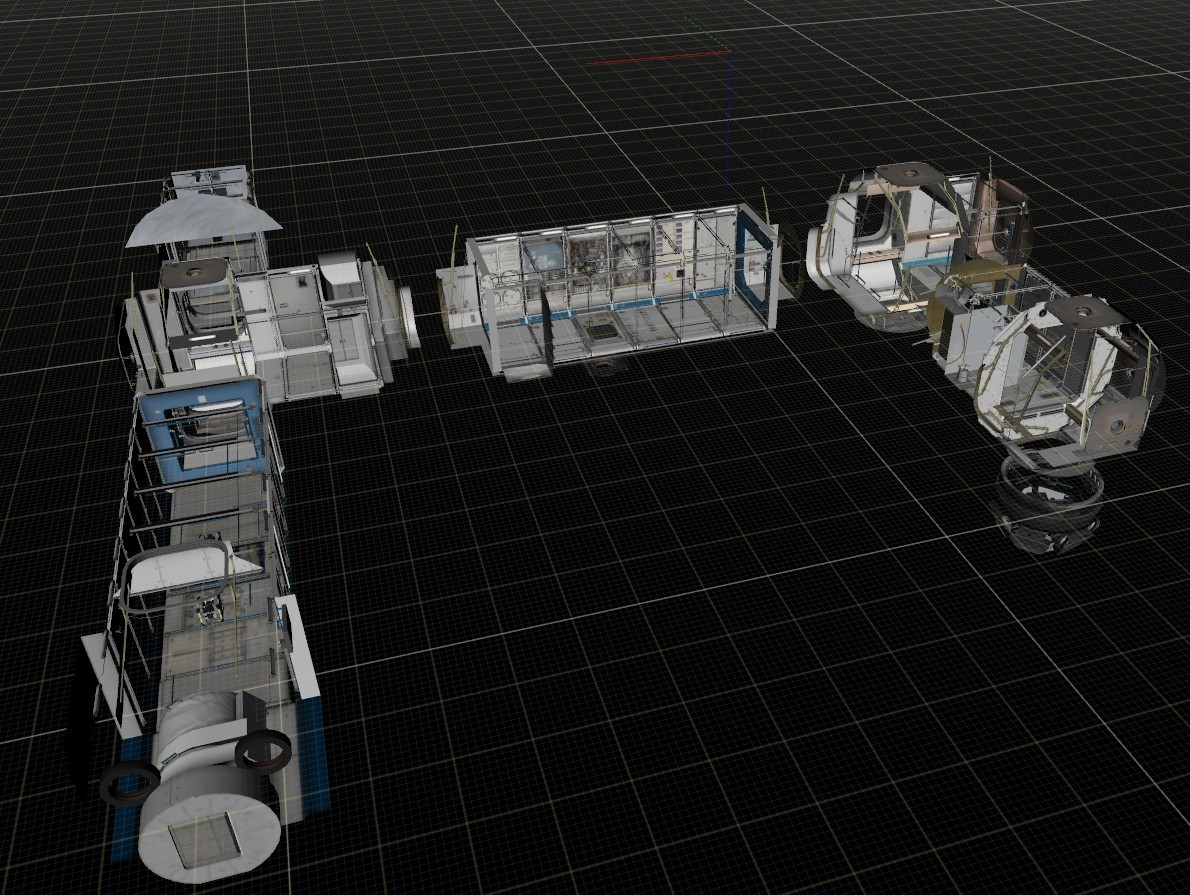
\includegraphics[width=0.8\textwidth]{img/ISS_env.jpg}
	\caption{The ISS simulation environment.}
\end{figure}

\begin{figure}[h!]
	\centering
	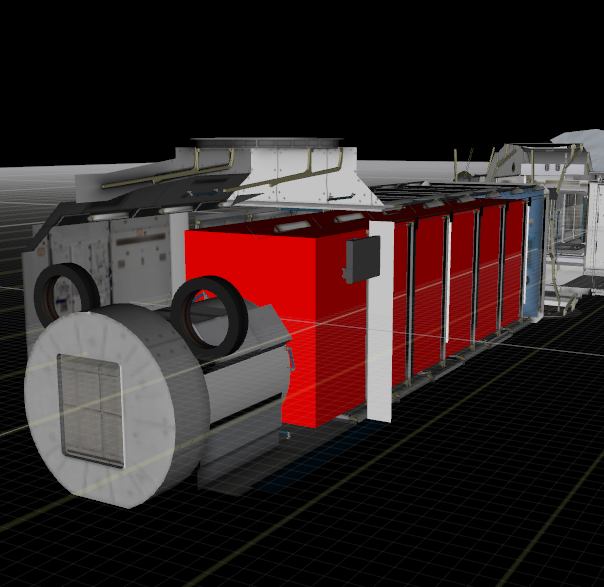
\includegraphics[width=0.8\textwidth]{img/ISS_volume.png}
	\caption{The approximate usable volume of the JEM, in red.}
\end{figure}


\subsection{The Astrobee Science Application Package (ASAP)}

The ASAP is the collection of source code and documentation that must be delivered to NASA for your project to be ISS-ready.

TODO

\subsection{Integration with GDS}

If using the default Astrobee Android route, GDS integration is as simple as creating custom commands for the Guest Science interface and receiving them properly in your code. However, if planning to run directly on the MLP/LLP it is necessary to intercept custom commands for use on the MLP/LLP. TODO: How to intercept.

\bibliography{bib.bib}
\bibliographystyle{plain}
\newpage

\appendix
\section{Directory Organization}

The entire directory breakdown is very long, but most important folders are noted here. Deeper descriptions for a few directories are available in the Doxygen documentation.\\

\begin{adjustwidth}{-1in}{-1in}
\begin{forest}
	for tree={
		font=\ttfamily,
		grow'=0,
		child anchor=west,
		parent anchor=south,
		anchor=west,
		calign=first,
		edge path={
			\noexpand\path [draw, \forestoption{edge}]
			(!u.south west) +(7.5pt,0) |- node[fill,inner sep=1.25pt] {} (.child anchor)\forestoption{edge label};
		},
		before typesetting nodes={
			if n=1
			{insert before={[,phantom]}}
			{}
		},
		fit=band,
		before computing xy={l=15pt},
	}
	[freeflyer
	[astrobee: "primary entry point" into the FSW: ROS looks here when roslaunch is called
	[config: configuration files for flight software]
	[launch: launches the flight software stack]
	[plans: holds plans which are built using the Ground Data System (GDS) user interface tool]
	[resources: all non-LUA resources used by nodes in the system]
	[scripts: bash script to print out the environment variables]
	]
	[cmake
	]
	[communications
	]
	[doc: tools for FSW documenation
	]
	[external
	]
	[gnc
	[ekf: extended Kalman Filter uses IMU and CV measurements from localization subsystem]
	[ctl: calculates forces and torques to meet requirements of mobility subsystem]
	[fam: force allocation module--this is like the SPHERES mixer]
	[sim: simulates the inputs to EKF robot's motion based on the outputs of FAM]
	[sim\_wrapper: ROS nodelets that convert inputs and outputs between ROS messages and Simulink]
	[gnc\_autocode: thin C++ wrapper around the auto-generated C functions]
	[matlab: the Matlab / Simulink code]
	]
	[hardware: drivers etc. for hardware control
	]
	[localization: feature detection algorithms which are then integrated into the EKF
	]
	[management: system monitoring and executive tools
	]
	]
\end{forest}
\newpage
\begin{forest}
	for tree={
		font=\ttfamily,
		grow'=0,
		child anchor=west,
		parent anchor=south,
		anchor=west,
		calign=first,
		edge path={
			\noexpand\path [draw, \forestoption{edge}]
			(!u.south west) +(7.5pt,0) |- node[fill,inner sep=1.25pt] {} (.child anchor)\forestoption{edge label};
		},
		before typesetting nodes={
			if n=1
			{insert before={[,phantom]}}
			{}
		},
		fit=band,
		before computing xy={l=15pt},
	}
	[freeflyer
	[mobility: tools that enable waypoint following within constraints
	[choreographer: accept and carry out motion requests from client nodes]
	[mapper: maintains a representation of the environment]
	[mobility: mobility tools]
	[planner\_qp: quartic polynomial planner]
	[planner\_trapezoidal: "straight line" planner]
	[sentinel: reacts to sensed data to check if likely to collide with an obstacle ]
	]
	[procedures: scripted procedures for typical maneuvers e.g. charge docking
	]
	[scripts: scripts for running FSW on the hardware
	]
	[shared: functions used between different packages
	]
	[simulation: all code related to the simulation
	[astrobee\_description: ROS URDFs used to describe Astrobee in simulation]
	[gazebo\_description: everything needed to run the Gazebo physics simulator
	[launch: load Gazebo; spawn Astrobee]
	[media: robot geometry; skins; etc.]
	[scripts]
	[src: plugins for the Gazebo simulator e.g. imu; nav cam]
	[worlds: describes the simulation environment e.g. ISS]
	]
	]
	[submodules: significantly large codebases used by Astrobee
	[android: Astrobee Android Guest Science API]
	[avionics]
	[common]
	[platform]
	]
	[tools: debugging tools that are not run during flight
	]
	[wdock
	]
	]
\end{forest}
\end{adjustwidth}

\section{ROS Tips}
So you want to mess with your ROS installation, huh? Luckily, adding and removing packages is often made very simple since packages are commonly packaged as debians and made available via apt. The typical naming convention is \begin{markdown}
	sudo apt-get install ros-DISTRIBUTION-PACKAGE_NAME
	
	sudo apt-get install ros-kinetic-rqt-logger-level
\end{markdown}
Make sure you run a \texttt{rosdep} to check any additional package requirements.

Occasionally, rostime will \textit{not} work at all after a shutdown of the Astrobee sim. This is a hard error to catch, and can be solved by restarting roscore.

\end{document}
